% Provenance (never printed): see sources/outline_sources.md (Year 2: Goldschmidt's
% classification; the chondritic Earth; core, mantle and crust compositions; trace
% elements and normalised diagrams). Curves from figdata/bachelor-2/geochem.py; exercise
% and problem values in the Book 4 scratch calculator calc/ch03.py.
\chapter{地球中的元素}\label{ch:b2:elements-in-the-earth}

大陆岩石每吨约含金
一点五毫克。上一章提到的\omterm{def:b2:planet-formation-meteorites:chondrule}{碳质球粒陨石}是最
原始的、从天而降的\omterm{def:b2:planet-formation-meteorites:fall-find}{陨石}，所含金约多一百倍。
地球正是由这类物质聚集而成，因此金并未从地球中缺失，
而是存在于别处。把地核与硅酸盐地球的估计成分
与地核质量结合起来计算，可知地球上超过 99\% 的金
位于地核之中，它随铁一同在地球
早期便沉入其中。金是一族元素中的一员，这族元素随金属
铁迁移；另一些随硫化物迁移，另一些随硅酸盐岩石，还有一些则逸入
空气。本章将元素按这些族进行划分，并利用
\omterm{def:b2:planet-formation-meteorites:chondrule}{球粒陨石}重建整个地球的成分并称量其
地核的质量，描述地幔、洋壳的成分，
陆壳的成分，并介绍\omterm{def:b2:elements-in-the-earth:trace}{微量元素}以及地球化学家
用来解读岩石历史的图解。
% ledger: rg03:ucc-trace, lodders:ci-table, mcd03:core, ms95:pm-trace, data:prem

\begin{recall}
地球具有金属地核，主要由铁组成，位于硅酸盐地幔和
薄地壳之下；地震学给出了各层的半径和密度，地核的
密度比相同压强与温度下的纯铁低 5\% 至 10\%，
这表明地核中含有轻元素：硅、硫、碳、
氧和氢是可能的候选者（本科一年级分册）。
元素的电负性表示其原子吸引成键电子的
能力强弱，离子半径取决于其电荷以及
近邻数目（化学系列本科一年级分册）。分配系数是
物质在两相中达到平衡时浓度之比，
（化学系列本科一年级分册）。\omterm{def:b2:planet-formation-meteorites:chondrule}{球粒陨石}、\omterm{def:b2:planet-formation-meteorites:chondrule}{碳质球粒陨石}
及\omterm{def:b2:planet-formation-meteorites:condensation}{凝聚序列}已在
\cref{ch:b2:planet-formation-meteorites}中介绍。
\end{recall}
% ledger: badro:core

\section{戈尔德施密特分类}

\omterm{def:b2:planet-formation-meteorites:chondrule}{球粒陨石}质天体熔化时，其物质分离为互不相溶的
液体：一种致密的铁镍金属、硫足量时形成的硫化物液体，以及
硅酸盐熔体，其上方为气相。每种元素按其化学性质在
这些相之间分配，同样的分配也见于
冶炼中，熔融铁、硫化锍与硅酸盐炉渣
在炉中分离。

\begin{definition}[戈尔德施密特分类]
\label{def:b2:elements-in-the-earth:goldschmidt}
\emph{戈尔德施密特分类}\index{戈尔德施密特分类}按元素在
分为金属、
硫化物、硅酸盐和气体的天体中所偏好的相来分类。
称偏好硅酸盐和氧化物者为\emph{亲石元素}\index{亲石元素}；
偏好金属铁者为\emph{亲铁元素}\index{亲铁元素}；
偏好硫化物者为\emph{亲铜元素}\index{亲铜元素}；
停留在气相中、以气体或挥发性化合物形式存在者为
\emph{亲气元素}\index{亲气元素}。
\end{definition}

这些类别遵循成键的化学规律。\omterm{def:b2:elements-in-the-earth:goldschmidt}{亲石元素}，例如
碱金属和碱土金属、铝、钛或\omterm{def:b2:elements-in-the-earth:ree}{稀土元素}，
容易把其电子交给电负性远更强的氧，
并与之形成离子键。\omterm{def:b2:elements-in-the-earth:goldschmidt}{亲铁元素}，即铂族金属、金、
镍和钴，其电负性接近铁，与氧的成键较弱，
并溶解于金属之中。\omterm{def:b2:elements-in-the-earth:goldschmidt}{亲铜元素}，如铜、锌、铅、
银和镉等，与硫形成的键具有更强的共价性。
\omterm{def:b2:elements-in-the-earth:goldschmidt}{亲气元素}包括稀有气体、氮和氢。许多
元素依条件不同可归属于两类：铁本身在富金属天体中
为\omterm{def:b2:elements-in-the-earth:goldschmidt}{亲铁元素}，而在氧化的地幔中为\omterm{def:b2:elements-in-the-earth:goldschmidt}{亲石元素}，
赋存于橄榄石和辉石中；钨和钼在地球中属\omterm{def:b2:elements-in-the-earth:goldschmidt}{亲铁元素}，
但其中大部分仍留在地幔中（见下图）。

\begin{omfigure}
\centering
\begin{tikzpicture}[x=0.62cm, y=-0.62cm,
  lith/.style={fill=brown!30}, sid/.style={fill=blue!30!gray!45},
  chal/.style={fill=orange!45}, atm/.style={fill=cyan!15}, none/.style={fill=black!8},
  cell/.style={draw=black!55, minimum size=0.58cm, inner sep=0pt, font=\scriptsize}]
\foreach \s/\c/\r/\k in {H/1/1/atm, He/18/1/atm,
  Li/1/2/lith, Be/2/2/lith, B/13/2/lith, C/14/2/atm, N/15/2/atm, O/16/2/lith,
  F/17/2/lith, Ne/18/2/atm,
  Na/1/3/lith, Mg/2/3/lith, Al/13/3/lith, Si/14/3/lith, P/15/3/lith, S/16/3/chal,
  Cl/17/3/lith, Ar/18/3/atm,
  K/1/4/lith, Ca/2/4/lith, Sc/3/4/lith, Ti/4/4/lith, V/5/4/lith, Cr/6/4/lith,
  Mn/7/4/lith, Fe/8/4/sid, Co/9/4/sid, Ni/10/4/sid, Cu/11/4/chal, Zn/12/4/chal,
  Ga/13/4/chal, Ge/14/4/sid, As/15/4/chal, Se/16/4/chal, Br/17/4/lith, Kr/18/4/atm,
  Rb/1/5/lith, Sr/2/5/lith, Y/3/5/lith, Zr/4/5/lith, Nb/5/5/lith, Mo/6/5/sid,
  Tc/7/5/none, Ru/8/5/sid, Rh/9/5/sid, Pd/10/5/sid, Ag/11/5/chal, Cd/12/5/chal,
  In/13/5/chal, Sn/14/5/chal, Sb/15/5/chal, Te/16/5/chal, I/17/5/lith, Xe/18/5/atm,
  Cs/1/6/lith, Ba/2/6/lith, Hf/4/6/lith, Ta/5/6/lith, W/6/6/sid, Re/7/6/sid,
  Os/8/6/sid, Ir/9/6/sid, Pt/10/6/sid, Au/11/6/sid, Hg/12/6/chal, Tl/13/6/chal,
  Pb/14/6/chal, Bi/15/6/chal, Po/16/6/none, At/17/6/none, Rn/18/6/none,
  La/3/8/lith, Ce/4/8/lith, Pr/5/8/lith, Nd/6/8/lith, Pm/7/8/none, Sm/8/8/lith,
  Eu/9/8/lith, Gd/10/8/lith, Tb/11/8/lith, Dy/12/8/lith, Ho/13/8/lith,
  Er/14/8/lith, Tm/15/8/lith, Yb/16/8/lith, Lu/17/8/lith,
  Th/4/9/lith, U/6/9/lith}
  \node[cell, \k] at (\c,\r) {\s};
\node[cell, lith, minimum width=0.58cm] at (3,6) {\tiny La--Lu};
\draw[black!50, -latex] (3,6.32) -- (3,7.65);
% legend
\foreach \k/\t/\x/\y in {lith/亲石/3.6/1, sid/亲铁/3.6/2,
  chal/亲铜/3.6/3, atm/亲气/7.8/1, none/{无稳定同位素}/7.8/2}
  \node[cell, \k, label={[font=\scriptsize]east:\t}] at (\x,\y) {};
\end{tikzpicture}
\par\smallskip{\small 稳定元素以及钍和铀（其长寿命同位素自地球形成之初延续至今）的戈尔德施密特类别，按
在地球中占主导的类别着色；\omterm{def:b2:elements-in-the-earth:ree}{稀土元素}位于方框
La--Lu 中。若干元素属于两类：铁、镍和钴在
氧化的地幔中也是\omterm{def:b2:elements-in-the-earth:goldschmidt}{亲石元素}；碳也是\omterm{def:b2:elements-in-the-earth:goldschmidt}{亲铁元素}，磷在
\omterm{def:b2:planet-formation-meteorites:fall-find}{陨石}中是\omterm{def:b2:elements-in-the-earth:goldschmidt}{亲铁元素}。}
\end{omfigure}

\section{球粒陨石地球}

没有人能整体采样地球：地核遥不可及，
地幔也只有碎块出露于地表。因此，整个地球的成分
需由两类证据构建：一是\omterm{def:b2:planet-formation-meteorites:fall-find}{陨石}，它们取样于行星形成所用的物质；
二是地幔岩石，
以及由地幔产生的熔体。

\begin{definition}[CI 球粒陨石]\label{def:b2:elements-in-the-earth:ci}
称\emph{CI 球粒陨石}\index{CI 球粒陨石}为以伊武纳\omterm{def:b2:planet-formation-meteorites:fall-find}{陨石}命名的
\omterm{def:b2:planet-formation-meteorites:chondrule}{碳质球粒陨石}群的一员：黑色、易碎的石块，
几乎完全由细粒基质构成，富含含水矿物和
碳，几乎不含球粒。除氢、碳、氮、氧及
稀有气体外，其成分在所有已知物质中最接近
太阳光球的成分；它们是地球化学的参考成分。
\end{definition}

该群共五颗\omterm{def:b2:planet-formation-meteorites:fall-find}{陨石}，均为目击坠落：Alais（1806）、Orgueil
（1864）、Tonk（1911）、Ivuna（1938）和 Revelstoke（1965）；Orgueil 最大，
重十四千克。该群采用的成分是加权平均值，
逐元素对其分析结果取平均；本章所用数值
在需要处引用。
% ledger: lodders:ci-table

\begin{definition}[难熔元素与挥发性元素]
\label{def:b2:elements-in-the-earth:volatility}
称\emph{难熔元素}\index{难熔元素}为其 50\% \omterm{def:b2:planet-formation-meteorites:condensation}{凝聚温度}
（\cref{ch:b2:planet-formation-meteorites}）高于
镁、硅和铁的\omterm{def:b2:planet-formation-meteorites:condensation}{凝聚温度}，即 \qtyrange{1310}{1340}{K}，
在 \qty{e-4}{bar} 下；
称\emph{挥发性元素}\index{挥发性元素}为\omterm{def:b2:planet-formation-meteorites:condensation}{凝聚温度}
低于上述各元素者。
\end{definition}

镁含量可作为标尺。镁是\omterm{def:b2:elements-in-the-earth:goldschmidt}{亲石元素}，
与岩石主体一同凝结，不进入地核，因此某元素与镁之比
在硅酸盐地球中的值除以其在 \omterm{def:b2:elements-in-the-earth:ci}{CI 球粒陨石}中的同一比值，
度量硅酸盐地球相对于
\omterm{def:b2:planet-formation-meteorites:chondrule}{球粒陨石}起始物质保留了该元素的多少。水、碳及其他挥发性化合物，
即 \omterm{def:b2:elements-in-the-earth:ci}{CI 球粒陨石}所含而地球未能保留的部分，在该比值中相互抵消。

\begin{definition}[全硅酸盐地球、原始地幔]
\label{def:b2:elements-in-the-earth:bse}
称\emph{全硅酸盐地球}\index{全硅酸盐地球}为地核之外的地球，
即地幔、地壳、海洋与大气的总和，视作已充分混合。
该成分亦称为\emph{原始地幔}\index{原始地幔}：
地核形成之后、尚未有任何地壳从中
抽取出来时的地幔。
\end{definition}

\omterm{def:b2:elements-in-the-earth:bse}{原始地幔}的估计依赖于那些失去熔体最少的地幔岩，
即熔岩携带至地表的捕掳体橄榄岩（下图为照片）或
出露于山脉中的橄榄岩，并假定难熔\omterm{def:b2:elements-in-the-earth:goldschmidt}{亲石元素}
彼此之间保持\omterm{def:b2:planet-formation-meteorites:chondrule}{球粒陨石}的比例。一项广泛使用的结果，
其镁、硅和铁的质量分数分别为 22.8\%、21.0\% 和 6.26\%，
列于后文的成分表中。
% ledger: ms95:pm-trace, ms95:pm-oxides

\begin{omfigure}
\centering
\begin{minipage}{0.48\linewidth}
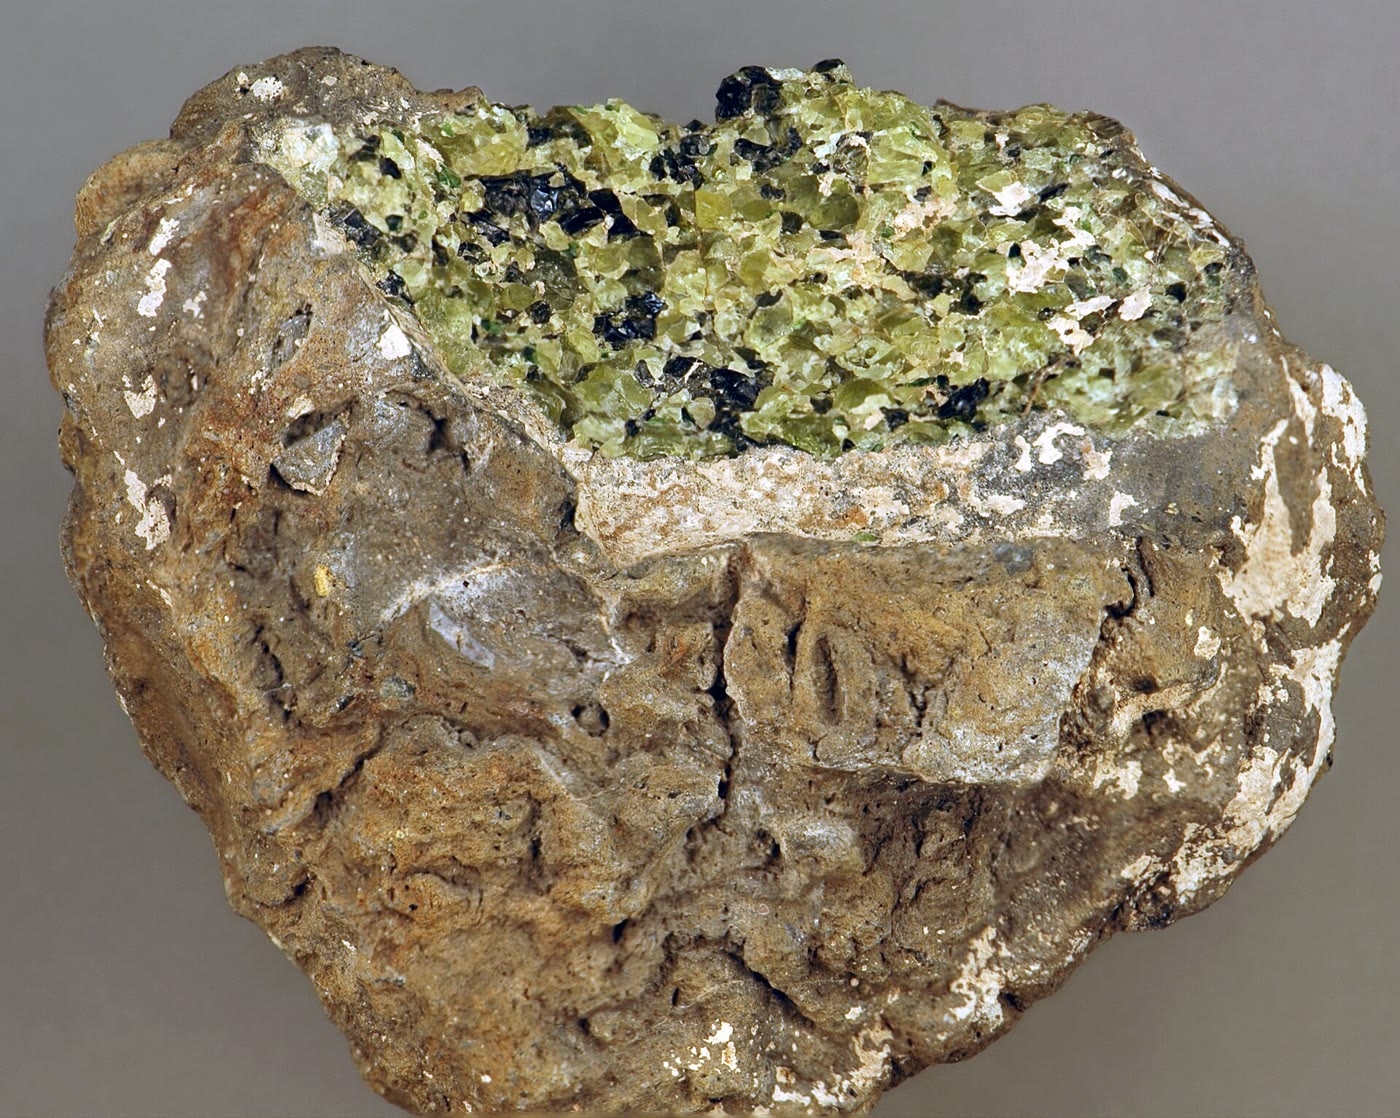
\includegraphics[width=\linewidth]{images/book4/b2-lherzolite-xenolith.jpg}
\end{minipage}\hfill
\begin{minipage}{0.48\linewidth}
{\small 取自新墨西哥州 Kilbourne Hole 玄武岩熔岩中的一块地幔橄榄岩（二辉橄榄岩）结核，
最宽处直径为 \qty{7.4}{cm}：黄绿色的
橄榄石与暗色辉石。熔岩将其从上地幔撕裂，
并携带至地表。James St.~John, CC BY 2.0。}
\end{minipage}
\end{omfigure}

下图将此硅酸盐地球与 \omterm{def:b2:elements-in-the-earth:ci}{CI 球粒陨石}逐元素比较，
并以上一章的\omterm{def:b2:planet-formation-meteorites:condensation}{凝聚温度}为横坐标。它以
其他证据都无法做到的方式为元素排序。难熔\omterm{def:b2:elements-in-the-earth:goldschmidt}{亲石元素}，
从锆和\omterm{def:b2:elements-in-the-earth:ree}{稀土元素}到锶和钡，它们
处于同一水平，彼此相差不超过 20\%：硅酸盐地球
保留了它们全部的\omterm{def:b2:planet-formation-meteorites:chondrule}{球粒陨石}比例。挥发性\omterm{def:b2:elements-in-the-earth:goldschmidt}{亲石元素}
随\omterm{def:b2:planet-formation-meteorites:condensation}{凝聚温度}降低而下降：钾和钠约存留五分之一，
铷约存留十分之一，氯约存留百分之一，溴和碘则
仅余千分之几。\omterm{def:b2:elements-in-the-earth:goldschmidt}{亲铁元素}远低于每一种
同挥发性的\omterm{def:b2:elements-in-the-earth:goldschmidt}{亲石元素}：硅酸盐地球保留的铁仅为其份额的七分之一，
镍为十三分之一，铂族金属和金约为
千分之三。这些元素进入了地核。\omterm{def:b2:elements-in-the-earth:goldschmidt}{亲铜元素}，
其中多数亦为挥发性的，两方面皆大幅亏损。

\begin{omfigure}
\centering
\begin{tikzpicture}
\begin{axis}[omrecord, width=0.95\linewidth, height=8.2cm, ymode=log,
  xmin=500, xmax=1800, ymin=8e-4, ymax=3, x dir=reverse,
  xlabel={\qty{e-4}{bar} 下的 50\% 凝聚温度 (K)},
  ylabel={$(X/\mathrm{Mg})_{\mathrm{BSE}}\,/\,(X/\mathrm{Mg})_{\mathrm{CI}}$},
  legend pos=south west, legend cell align=left, legend style={font=\scriptsize},
  tick label style={font=\scriptsize}, label style={font=\small},
  scaled x ticks=false, xticklabel style={/pgf/number format/1000 sep={}}]
\addplot[black!40, dashed, domain=500:1800, samples=2, forget plot] {1};
\addplot[only marks, mark=*, mark size=1.6pt, brown!70!black]
  table[x=T, y=ratio] {figdata/out/bachelor-2-geochem-volat-lith.dat};
\addlegendentry{亲石元素}
\addplot[only marks, mark=square*, mark size=1.6pt, blue!60!black]
  table[x=T, y=ratio] {figdata/out/bachelor-2-geochem-volat-sid.dat};
\addlegendentry{亲铁元素}
\addplot[only marks, mark=triangle*, mark size=2pt, orange!80!black]
  table[x=T, y=ratio] {figdata/out/bachelor-2-geochem-volat-chal.dat};
\addlegendentry{亲铜元素}
\node[font=\tiny, brown!50!black, anchor=south] at (axis cs:1600,1.35)
  {Zr, Hf, Al, Sc, Y, Th, U, Ti, Ca, Sr, Ba, 稀土元素};
\begin{scope}[font=\tiny, brown!50!black]
\node[anchor=west] at (axis cs:1328,1.0) {Mg};
\node[anchor=north] at (axis cs:1310,0.80) {Si};
\node[anchor=west] at (axis cs:1150,0.23) {Mn};
\node[anchor=south] at (axis cs:1142,0.47) {Li};
\node[anchor=south] at (axis cs:1010,0.195) {K};
\node[anchor=north] at (axis cs:958,0.22) {Na};
\node[anchor=north] at (axis cs:908,0.175) {B};
\node[anchor=north] at (axis cs:800,0.116) {Rb};
\node[anchor=south] at (axis cs:734,0.175) {F};
\node[anchor=west] at (axis cs:795,0.0477) {Cs};
\node[anchor=west] at (axis cs:944,0.0102) {Cl};
\node[anchor=north] at (axis cs:546,0.0061) {Br};
\node[anchor=south] at (axis cs:535,0.0088) {I};
\end{scope}
\begin{scope}[font=\tiny, blue!50!black]
\node[anchor=west] at (axis cs:1325,0.144) {Fe};
\node[anchor=east] at (axis cs:1364,0.0775) {Ni};
\node[anchor=west] at (axis cs:1342,0.088) {Co};
\node[anchor=west] at (axis cs:1780,0.137) {W};
\node[anchor=south] at (axis cs:1590,0.0206) {Mo};
\node[anchor=north] at (axis cs:883,0.0139) {Ge};
\node[anchor=north] at (axis cs:1500,0.0026) {Re, Os, Ir, Ru, Pt, Pd};
\node[anchor=north] at (axis cs:1060,0.0026) {Au};
\end{scope}
\begin{scope}[font=\tiny, orange!60!black]
\node[anchor=west] at (axis cs:1030,0.0993) {Cu};
\node[anchor=north] at (axis cs:996,0.0167) {Ag};
\node[anchor=south] at (axis cs:726,0.0746) {Zn};
\node[anchor=south] at (axis cs:704,0.0325) {Sn};
\node[anchor=east] at (axis cs:735,0.0246) {Pb};
\node[anchor=west] at (axis cs:648,0.0249) {Cd};
\node[anchor=east] at (axis cs:715,0.0022) {Te};
\node[anchor=north] at (axis cs:690,0.0016) {Se};
\node[anchor=west] at (axis cs:660,0.0019) {S};
\end{scope}
\end{axis}
\end{tikzpicture}
\par\smallskip{\small 硅酸盐地球与 \omterm{def:b2:elements-in-the-earth:ci}{CI 球粒陨石}的比较：对每一元素 $X$，
\omterm{def:b2:elements-in-the-earth:bse}{全硅酸盐地球}中的比值 $X/\mathrm{Mg}$ 除以 \omterm{def:b2:elements-in-the-earth:ci}{CI 球粒陨石}中的同一比值，
对 50\% \omterm{def:b2:planet-formation-meteorites:condensation}{凝聚温度}（高温在左）作图。
难熔\omterm{def:b2:elements-in-the-earth:goldschmidt}{亲石元素}彼此之间与\omterm{def:b2:planet-formation-meteorites:chondrule}{球粒陨石}一致；\omterm{def:b2:elements-in-the-earth:volatility}{挥发性
元素}随\omterm{def:b2:planet-formation-meteorites:condensation}{凝聚温度}降低而亏损；\omterm{def:b2:elements-in-the-earth:goldschmidt}{亲铁元素}与
\omterm{def:b2:elements-in-the-earth:goldschmidt}{亲铜元素}则亏损得更为严重。数据来源：McDonough and Sun (1995)；
Lodders (2003)。}
\end{omfigure}
% ledger: ms95:pm-trace, lodders:ci-table, lodders:tc-table, lodders:tc-more

难熔\omterm{def:b2:elements-in-the-earth:goldschmidt}{亲石元素}的含量比镁约高 15\%。
二者不可能同时与\omterm{def:b2:planet-formation-meteorites:chondrule}{球粒陨石}精确一致：要么地球获得了\omterm{def:b2:elements-in-the-earth:volatility}{难熔
元素}，要么地球损失了少量镁，要么模型中镁的含量被
低估（见\cref{exo:b2:elements-in-the-earth:12}）。硅的比值为 0.83，距难熔水平差得更远，
部分缺失的硅可能位于地核中（练习）。

硅酸盐地球中的\omterm{def:b2:elements-in-the-earth:goldschmidt}{亲铁元素}，与\omterm{def:b2:planet-formation-meteorites:chondrule}{球粒陨石}型全地球
组合起来，可以称出地核的质量。设全地球的 CI 比值为 $r_X = X/\mathrm{Mg}$
对\omterm{def:b2:elements-in-the-earth:goldschmidt}{亲铁元素} $X$，地核中该元素的浓度为 $c_X$，
但地核中不含镁。

\begin{proposition}[由球粒陨石比值求地核质量分数]
\label{prop:b2:elements-in-the-earth:core}
设 $x$ 为地核的质量分数，$C_X$ 与 $C_{\mathrm{Mg}}$ 分别为
硅酸盐地球中 $X$ 与镁的浓度，$c_X$ 为 $X$ 在
地核中的浓度。若地球具有\omterm{def:b2:planet-formation-meteorites:chondrule}{球粒陨石}比值 $r_X$，则
\[
  \frac{x}{1-x} = \frac{r_X C_{\mathrm{Mg}} - C_X}{c_X}.
\]
\end{proposition}

\begin{proof}
质量为 $M$ 的地球，含有 $(1-x)MC_X + xMc_X$ 的 $X$，
以及 $(1-x)MC_{\mathrm{Mg}}$ 的镁。二者之比为 $r_X$：
即 $(1-x)C_X + xc_X = r_X(1-x)C_{\mathrm{Mg}}$。两边除以 $(1-x)c_X$，
即得结论。
\end{proof}

对于铁，在 \omterm{def:b2:elements-in-the-earth:ci}{CI 球粒陨石}中，$r_{\mathrm{Fe}} = \num{182800}/\num{95870} = 1.907$，
硅酸盐地球中镁占 22.8\%，铁占 6.26\%，模型地核中
铁占 85.5\%，由命题得 $x/(1-x) = 0.435$，地核占
地球质量的 30\%。地震学依据地球参考模型的密度积分，
得出 32.5\%。两者在一成之内吻合，
支持地球为\omterm{def:b2:planet-formation-meteorites:chondrule}{球粒陨石}型、铁主要位于地核中的图景；两者之差
度量地球铁镁比偏离\omterm{def:b2:planet-formation-meteorites:chondrule}{球粒陨石}比值的程度
（练习）。同一平衡也说明地球各元素的分布
（见下图）：几乎全部的铂、铱与金，以及大部分的铁、
镍与硫，都位于地核中。
% ledger: lodders:ci-table, ms95:pm-trace, mcd03:core, data:prem

\begin{omfigure}
\centering
\begin{tikzpicture}
\begin{axis}[omrecord, xbar, width=0.8\linewidth, height=6.4cm, bar width=5pt,
  xmin=0, xmax=100, ymin=0.4, ymax=14.6, y dir=reverse,
  ytick={1,...,14}, yticklabels={{Ir},{Pt},{Au},{Mo},{S},{Ni},{W},{Fe},{Cr},{Si},{Mg},{Al},{Ca},{K}},
  xlabel={地核中所含地球储量的份额（\%）},
  tick label style={font=\scriptsize}, label style={font=\small},
  nodes near coords, nodes near coords align={horizontal},
  every node near coord/.append style={font=\tiny, /pgf/number format/fixed,
    /pgf/number format/precision=1}]
\addplot[fill=blue!35!gray!50, draw=black!60]
  table[x=share, y=idx] {figdata/out/bachelor-2-geochem-budget.dat};
\end{axis}
\end{tikzpicture}
\par\smallskip{\small 地球各元素的去向：每种元素在地核中所占的份额，
由模型地核成分、\omterm{def:b2:elements-in-the-earth:bse}{原始地幔}，以及地核占地球 32.5\%
质量的假设推算。数据来源：McDonough (2003)；McDonough and Sun (1995)；
地球参考模型。}
\end{omfigure}
% ledger: mcd03:core, ms95:pm-trace, data:prem

\section{地幔与地壳}

硅酸盐地球自形成以来，已分化为地幔与两
类地壳。洋壳由洋中脊下方地幔的熔融形成；
陆壳则经长期在俯冲带之上的熔融、
再造与侵蚀而成（见后续章节）。
地幔的两种参考熔体为讨论提供了依据。

\begin{definition}[洋中脊玄武岩，洋岛玄武岩]
\label{def:b2:elements-in-the-earth:morb-oib}
称\emph{洋中脊玄武岩}\index{洋中脊玄武岩}（MORB）为在洋中脊喷发的玄武岩，
即洋壳顶部的岩石。称
\emph{洋岛玄武岩}\index{洋岛玄武岩}（OIB）为在远离板块边界的
海洋火山喷发的玄武岩，如夏威夷的
火山所产，通常认为与地幔柱有关（本科一年级分册）。
\end{definition}

下表中的平均 MORB 为全球平均值，由 771 个洋脊
段构成，每段按其长度与扩张速率加权，使平均值
代表洋脊所产生的洋壳。OIB
列为单一岩石：玄武岩标准物质 BHVO-2，于 1995 年
采自 1919 年溢出于夏威夷基拉韦厄火山哈雷马乌马乌火山口的熔岩，
并经多家实验室分析，因而其大部分\omterm{def:b2:elements-in-the-earth:ree}{稀土元素}含量已知到
约 1\% 的精度。上陆壳是由地表岩石与沉积物
估算得到的平均成分。
% ledger: gale13:allmorb, usgs:bhvo2-origin, usgs:bhvo2-major, rg14:crust

\begin{table}[h]
\centering
\small
\begin{tabular}{lrrrr}
\hline
氧化物 (wt\,\%) & \omterm{def:b2:elements-in-the-earth:bse}{原始地幔} & MORB & OIB (BHVO-2) & 上陆壳 \\
\hline
\ce{SiO2} & 45.0 & 50.47 & 49.60 & 66.6\\
\ce{TiO2} & 0.201 & 1.68 & 2.731 & 0.64\\
\ce{Al2O3} & 4.45 & 14.70 & 13.44 & 15.4\\
FeO （总量） & 8.05 & 10.43 & 11.15 & 5.04\\
MnO & 0.135 & 0.184 & 0.1690 & 0.10\\
MgO & 37.8 & 7.58 & 7.257 & 2.48\\
CaO & 3.55 & 11.39 & 11.40 & 3.59\\
\ce{Na2O} & 0.36 & 2.79 & 2.219 & 3.27\\
\ce{K2O} & 0.029 & 0.160 & 0.5130 & 2.80\\
\ce{P2O5} & 0.021 & 0.184 & 0.2685 & 0.15\\
\hline
\end{tabular}
\caption{四个储库的主量元素组成。BHVO-2 中的铁以
\ce{Fe2O3} 形式给出（12.39\%），此处换算为 FeO。数据来源：McDonough and Sun
(1995)；Gale 等人（2013）；BHVO-2 的 USGS 信息单；Rudnick and
Gao (2014)。}
\label{tab:b2:elements-in-the-earth:majors}
\end{table}
% ledger: ms95:pm-oxides, gale13:allmorb, usgs:bhvo2-major, rg14:crust

横向读此表，可看出熔融的故事。地幔是富镁的
橄榄岩，MgO 含量接近 38\%，\ce{Al2O3} 与 CaO 均低于 5\%。
其熔体即玄武岩，镁的含量仅为地幔的五分之一，而
钙和铝的含量则为其三倍：易进入熔体的元素
最先离开地幔。与地幔相比，钾、钠和钛在熔体中
的含量更高，而钾在大陆地壳中含量最高，
约为其在\omterm{def:b2:elements-in-the-earth:bse}{原始地幔}中浓度的近百倍。硅从地幔到
玄武岩的升高很小，在大陆地壳中则升高得多，
其平均值接近花岗闪长岩。

\section{微量元素}

十种氧化物约占上表中每种岩石的 99\%。其余元素
含量在百万分之几的量级，与主量元素遵循相同的过程，但
对这些过程的敏感性要强得多。

\begin{definition}[微量元素]\label{def:b2:elements-in-the-earth:trace}
岩石中的\emph{微量元素}\index{微量元素}是指其浓度
按质量计通常低于 0.1\%（\qty{1000}{ppm}）的元素。
微量元素很少自成矿物，
而是替代晶格位置上的主量元素。
\end{definition}

\omterm{def:b2:elements-in-the-earth:trace}{微量元素}的含量极低，其自身浓度不会改变晶体或熔体；
因此它在两者之间的分配是一个简单的比值，
在较宽的浓度范围内与其浓度无关。

\begin{definition}[矿物–熔体分配系数；相容元素和
不相容元素]\label{def:b2:elements-in-the-earth:partition}
称某元素在某矿物中的\emph{矿物–熔体分配系数}\index{矿物–熔体分配系数}
为该元素在矿物中的浓度与其
在与之平衡的硅酸盐熔体中浓度之比，
$D = C_{\mathrm{mineral}}/C_{\mathrm{melt}}$。若岩石由若干矿物组成，质量分数分别为
$x_i$，则\emph{总分配系数}为
$\bar D = C_{\mathrm{rock}}/C_{\mathrm{melt}}$。某元素在岩石中
为\emph{相容元素}\index{相容元素}，条件是 $\bar D > 1$；
若 $\bar D < 1$，则为\emph{不相容元素}\index{不相容元素}。
\end{definition}

\begin{proposition}[总分配系数]
\label{prop:b2:elements-in-the-earth:bulk-d}
若岩石中每种矿物都与同一熔体平衡，则
总分配系数为各矿物分配系数的加权平均，权重为质量分数：
$\bar D = \sum_i x_i D_i$。
\end{proposition}

\begin{proof}
岩石的浓度为 $C_{\mathrm{rock}} = \sum_i x_i C_i$，且每种矿物
满足 $C_i = D_i C_{\mathrm{melt}}$。两边除以 $C_{\mathrm{melt}}$ 即得结论。
\end{proof}

离子能否进入某一位置，取决于其半径和电荷。与某位置主要离子半径和电荷相近的离子，
例如在橄榄石中以 \ce{Ni^2+} 替代 \ce{Mg^2+}，
易于进入，是相容的。半径大得多的离子，例如
\ce{Rb+} 或 \ce{Ba^2+}，或电荷更高的离子，例如 \ce{Zr^4+} 或
\ce{Nb^5+}，会使晶格受力而被排斥进入熔体：在地幔矿物中是不相容的。
\omterm{def:b2:elements-in-the-earth:partition}{不相容元素}中有两组，在有水参与时行为不同，
将在后文讨论。

\begin{definition}[大离子亲石元素与高场强元素]
\label{def:b2:elements-in-the-earth:lile-hfse}
称\emph{大离子亲石元素}\index{大离子亲石元素}
（LILE）是指带低电荷（$+1$ 或 $+2$）大离子的\omterm{def:b2:elements-in-the-earth:partition}{不相容元素}：
钾、铷、铯、锶、钡。
称\emph{高场强元素}\index{高场强元素}（HFSE）
是指小半径、高电荷（$+4$ 或 $+5$）离子的\omterm{def:b2:elements-in-the-earth:partition}{不相容元素}：
锆、铪、铌、钽、钛。
\end{definition}

LILE 易溶于富水流体，HFSE 则几乎不溶解。
经水蚀变的岩石，或继承了上文所述俯冲带流体的熔体，
因此携带 LILE 多而 HFSE 少。

\begin{definition}[稀土元素]\label{def:b2:elements-in-the-earth:ree}
\emph{稀土元素}\index{稀土元素}（REE）是指十五种镧系元素，
即从镧到镥，钷没有稳定同位素。所有
元素均为\omterm{def:b2:elements-in-the-earth:goldschmidt}{亲石元素}和\omterm{def:b2:elements-in-the-earth:volatility}{难熔元素}，几乎都是三价，其离子半径
从镧到镥稳定减小；铕在
还原性熔体中也可呈二价。
\end{definition}

由于\omterm{def:b2:elements-in-the-earth:ree}{稀土元素}只在半径上平滑变化，
它们的分异也平滑进行：轻稀土（从镧到钐）的相容性最弱；
重稀土（从钆到镥）更易进入某些
矿物，尤其是石榴子石（见下图）。含石榴子石的岩石中，重稀土
变为\omterm{def:b2:elements-in-the-earth:partition}{相容元素}：这种岩石的熔体富含轻稀土，
而重稀土含量低。

\begin{omfigure}
\centering
\begin{tikzpicture}
\begin{axis}[omrecord, width=0.78\linewidth, height=6.4cm, ymode=log,
  xmin=0.6, xmax=9.4, ymin=5e-4, ymax=20,
  xtick={1,...,9}, xticklabels={{La},{Ce},{Nd},{Sm},{Eu},{Gd},{Tb},{Yb},{Lu}},
  ylabel={分配系数 $D$}, legend pos=south east,
  legend cell align=left, legend style={font=\scriptsize},
  tick label style={font=\scriptsize}, label style={font=\small}]
\addplot[black!40, dashed, domain=0.6:9.4, samples=2, forget plot] {1};
\addplot[thick, green!45!black, mark=*] table[x=idx, y=cpx] {figdata/out/bachelor-2-geochem-dvals.dat};
\addlegendentry{单斜辉石}
\addplot[thick, red!70!black, mark=square*] table[x=idx, y=gar] {figdata/out/bachelor-2-geochem-dvals.dat};
\addlegendentry{石榴子石}
\addplot[thick, olive!70!black, mark=triangle*] table[x=idx, y=ol] {figdata/out/bachelor-2-geochem-dvals.dat};
\addlegendentry{橄榄石 + 斜方辉石 + 尖晶石}
\addplot[very thick, black, mark=diamond*] table[x=idx, y=bulk] {figdata/out/bachelor-2-geochem-dvals.dat};
\addlegendentry{全岩（65/18/17\%）}
\node[font=\scriptsize, anchor=south west] at (axis cs:0.7,1) {相容};
\node[font=\scriptsize, anchor=north west] at (axis cs:0.7,1) {不相容};
\end{axis}
\end{tikzpicture}
\par\smallskip{\small \omterm{def:b2:elements-in-the-earth:ree}{稀土元素}的\omterm{def:b2:elements-in-the-earth:partition}{矿物–熔体分配系数}，所示矿物为单斜辉石、石榴子石，
以及橄榄石、斜方辉石和尖晶石的混合物，并给出
由 65\% 单斜辉石、18\% 石榴子石及 17\% 其他矿物组成的
石榴辉石岩的总分配系数（见上文命题）。石榴子石使重稀土成为\omterm{def:b2:elements-in-the-earth:partition}{相容元素}。
数据来源：Budahn (1991)。}
\end{omfigure}
% ledger: budahn91:d-ree, budahn91:modes

\section{标准化图解}

相邻元素的丰度因物质的核历史而相差甚大：
偶原子序数元素的丰度高于其
奇原子序数的邻近元素，如\omterm{def:b2:elements-in-the-earth:ree}{稀土元素}的 CI 数据所示（镧 0.232，
铈 0.621，镨 0.0928 ppm）。直接作图时，岩石的\omterm{def:b2:elements-in-the-earth:ree}{稀土元素}呈
锯齿状，掩盖其地质历史。除以参考值即可消除此现象。
% ledger: lodders:ci-table

\begin{definition}[标准化图解]\label{def:b2:elements-in-the-earth:normalised}
称\emph{标准化图解}\index{标准化图解}为这样的图：对一系列按固定顺序排列的元素，
样品中的浓度与参考物中的浓度之比，
即 $X_N = C_X/C_X^{\mathrm{ref}}$，在对数坐标上作图。\omterm{def:b2:elements-in-the-earth:ree}{稀土元素}
以 \omterm{def:b2:elements-in-the-earth:ci}{CI 球粒陨石}为参考进行标准化，按原子序数排列；
较长的一组\omterm{def:b2:elements-in-the-earth:partition}{不相容元素}，常称蛛网图，以\omterm{def:b2:elements-in-the-earth:bse}{原始地幔}为参考
进行标准化，并按其在地幔熔融中的不相容性递减排列。
\end{definition}

与参考物比例相同的样品在图上呈水平线；
其高度给出富集程度。斜率反映轻元素与
重元素之间的分异，常以 $(\mathrm{La}/\mathrm{Yb})_N$ 之类的比值度量。
偏离直线的单个元素即为异常。

\begin{proposition}[铕异常]\label{prop:b2:elements-in-the-earth:normalised}
在\omterm{def:b2:elements-in-the-earth:normalised}{标准化图解}中，若图形在
$\log X_N$ 上钐与钆之间为一条直线时，位于中间的铕的期望值
为 $\mathrm{Eu}^* = \sqrt{\mathrm{Sm}_N\,\mathrm{Gd}_N}$。
\emph{铕异常}\index{铕异常}为
$\mathrm{Eu}/\mathrm{Eu}^* = \mathrm{Eu}_N/\sqrt{\mathrm{Sm}_N\,\mathrm{Gd}_N}$：
小于 1 为负，大于 1 为正。
\end{proposition}

\begin{proof}
钐、铕、钆在坐标轴上等距相邻。
在 $\log X_N$ 中，直线在中点处的值等于两端值的平均：
$\log \mathrm{Eu}^* = \tfrac12(\log \mathrm{Sm}_N + \log \mathrm{Gd}_N)$，
即为几何平均值的对数。
\end{proof}

铕是唯一可能呈二价的\omterm{def:b2:elements-in-the-earth:ree}{稀土元素}。\ce{Eu^2+} 的
离子半径与 \ce{Ca^2+}、\ce{Sr^2+} 相近，因此斜长石能接纳它，
同时排斥三价\omterm{def:b2:elements-in-the-earth:ree}{稀土元素}。析出斜长石后的熔体
具有负异常；残留的富斜长石岩石则为正异常。

\begin{omfigure}
\centering
\begin{tikzpicture}
\begin{axis}[omrecord, width=0.8\linewidth, height=6.4cm, ymode=log,
  xmin=0.6, xmax=13.4, ymin=5, ymax=250,
  xtick={1,...,13}, xticklabels={{La},{Ce},{Pr},{Nd},{Sm},{Eu},{Gd},{Tb},{Dy},{Ho},{Er},{Yb},{Lu}},
  ylabel={样品 / CI 球粒陨石}, legend pos=north east, legend cell align=left,
  legend style={font=\scriptsize}, tick label style={font=\scriptsize},
  label style={font=\small}]
\addplot[thick, blue!70!black, mark=*] table[x=idx, y=morb] {figdata/out/bachelor-2-geochem-ree.dat};
\addlegendentry{平均 MORB}
\addplot[thick, red!70!black, mark=square*] table[x=idx, y=oib] {figdata/out/bachelor-2-geochem-ree.dat};
\addlegendentry{OIB（BHVO-2，夏威夷）}
\addplot[thick, brown!70!black, mark=triangle*] table[x=idx, y=ucc] {figdata/out/bachelor-2-geochem-ree.dat};
\addlegendentry{上部陆壳}
\end{axis}
\end{tikzpicture}
\par\smallskip{\small 以 \omterm{def:b2:elements-in-the-earth:ci}{CI 球粒陨石}标准化的\omterm{def:b2:elements-in-the-earth:ree}{稀土元素}分布（略去铥，
因缺少 MORB 数值）。平均 MORB 近于平坦，轻稀土略低；
夏威夷玄武岩富集稀土；上部陆壳则强烈
富集稀土，并具负\omterm{prop:b2:elements-in-the-earth:normalised}{铕异常}。数据来源：Gale 等人
（2013）；USGS BHVO-2 数据表；Rudnick 和 Gao；Lodders（2003）。}
\end{omfigure}
% ledger: gale13:allmorb, usgs:bhvo2-trace, rg03:ucc-trace, lodders:ci-table

上图的三种配分模式可读作三段历史。平均 MORB
约高于\omterm{def:b2:planet-formation-meteorites:chondrule}{球粒陨石} 25 倍，近于平坦，其 $(\mathrm{La}/\mathrm{Sm})_N
= 0.85$：其地幔源区已将部分最\omterm{def:b2:elements-in-the-earth:partition}{不相容元素}
转移到较早的熔体中，其中包括陆壳。夏威夷玄武岩
富集轻稀土，$(\mathrm{La}/\mathrm{Yb})_N = 5.4$，其
重稀土低于 MORB，说明其来自较小程度的
熔融，残留的石榴子石保留了重稀土。上部
陆壳中镧富集超过百倍，且
$(\mathrm{La}/\mathrm{Yb})_N = 10.9$ 与 $\mathrm{Eu}/\mathrm{Eu}^* = 0.72$：它
是多次熔融的产物，其铕亏损与
深部地壳中残留的斜长石相符。

\begin{omfigure}
\centering
\begin{tikzpicture}
\begin{axis}[omrecord, width=\linewidth, height=6.6cm, ymode=log,
  xmin=0.5, xmax=27.5, ymin=1, ymax=400,
  xtick={1,...,27}, xticklabels={{Cs},{Rb},{Ba},{Th},{U},{Nb},{Ta},{K},{La},{Ce},{Pb},{Pr},{Sr},{Nd},{Zr},{Hf},{Sm},{Eu},{Ti},{Gd},{Tb},{Dy},{Y},{Ho},{Er},{Yb},{Lu}},
  ylabel={样品 / 原始地幔}, legend pos=north east, legend cell align=left,
  legend style={font=\scriptsize}, tick label style={font=\scriptsize},
  label style={font=\small}]
\addplot[thick, blue!70!black, mark=*, mark size=1.4pt] table[x=idx, y=morb] {figdata/out/bachelor-2-geochem-spider.dat};
\addlegendentry{平均 MORB}
\addplot[thick, red!70!black, mark=square*, mark size=1.4pt] table[x=idx, y=oib] {figdata/out/bachelor-2-geochem-spider.dat};
\addlegendentry{OIB（BHVO-2）}
\addplot[thick, brown!70!black, mark=triangle*, mark size=1.6pt] table[x=idx, y=ucc] {figdata/out/bachelor-2-geochem-spider.dat};
\addlegendentry{上部陆壳}
\end{axis}
\end{tikzpicture}
\par\smallskip{\small 以\omterm{def:b2:elements-in-the-earth:bse}{原始地幔}标准化的\omterm{def:b2:elements-in-the-earth:partition}{不相容元素}，自最不相容者起
排于左侧。陆壳显示出高 LILE 含量，并
在铌、钽、钛处出现深谷，以及继承自
俯冲带熔融的铅峰；夏威夷玄武岩在铌和
钽处呈隆起。钾和钛由氧化物换算。数据同\omterm{def:b2:elements-in-the-earth:ree}{稀土
元素}图；McDonough 和 Sun（1995）。}
\end{omfigure}
% ledger: gale13:allmorb, usgs:bhvo2-trace, usgs:bhvo2-major, rg03:ucc-trace, ms95:pm-trace

上图的蛛网图使对比更加鲜明。在陆壳中，
铌和钽远低于其邻元素钍和镧，
钛低于其邻元素，铅则明显偏高：$(\mathrm{Nb}/\mathrm{La})_N =
0.38$。夏威夷玄武岩中同一比值为 1.17，平均 MORB 中为
0.99。陆壳的该模式是俯冲带之上熔体的特征，
流体将 LILE 与铅带入地幔楔，而将 HFSE 留在其后
（后续章节再述）；\omterm{def:b2:elements-in-the-earth:morb-oib}{洋岛玄武岩}则无此特征。单个样品的蛛网图
因此可借此区分弧熔岩与洋岛熔岩，或揭示玄武岩
受大陆地壳混染（见\cref{exo:b2:elements-in-the-earth:11}）。

\begin{inthelab}[从岩石到微量元素表]
\begin{minipage}[t]{0.6\linewidth}
\vspace{0pt}
若地球化学家要测定一块玄武岩的\omterm{def:b2:elements-in-the-earth:trace}{微量元素}，他需从数百克
最新鲜的内部取样，去除风化外壳和矿脉。岩石先被破碎，
再在研磨机中磨成细粉，研磨机的材料不得
污染所关心的元素。取少量粉末，
用酸溶解，或与助熔剂熔融，再将溶液用电感耦合等离子体质谱法分析，
一次即可测得蛛网图中的大部分元素。
每批样品都要同时分析已知成分的参考物质，
例如夏威夷玄武岩 BHVO-2：其数值源自综合多家实验室均值的研究，
其中镧的数值来自 132 家实验室；部分数值，如钕和钐，
则由同位素稀释法获得，该法以已知加入量的某一同位素，
来计算元素的原子数。
若实验室对参考物质的测定结果落在公认值的
不确定度范围之内，未知样品的结果
随之被接受。
\end{minipage}\hfill
\begin{minipage}[t]{0.36\linewidth}
\vspace{0pt}
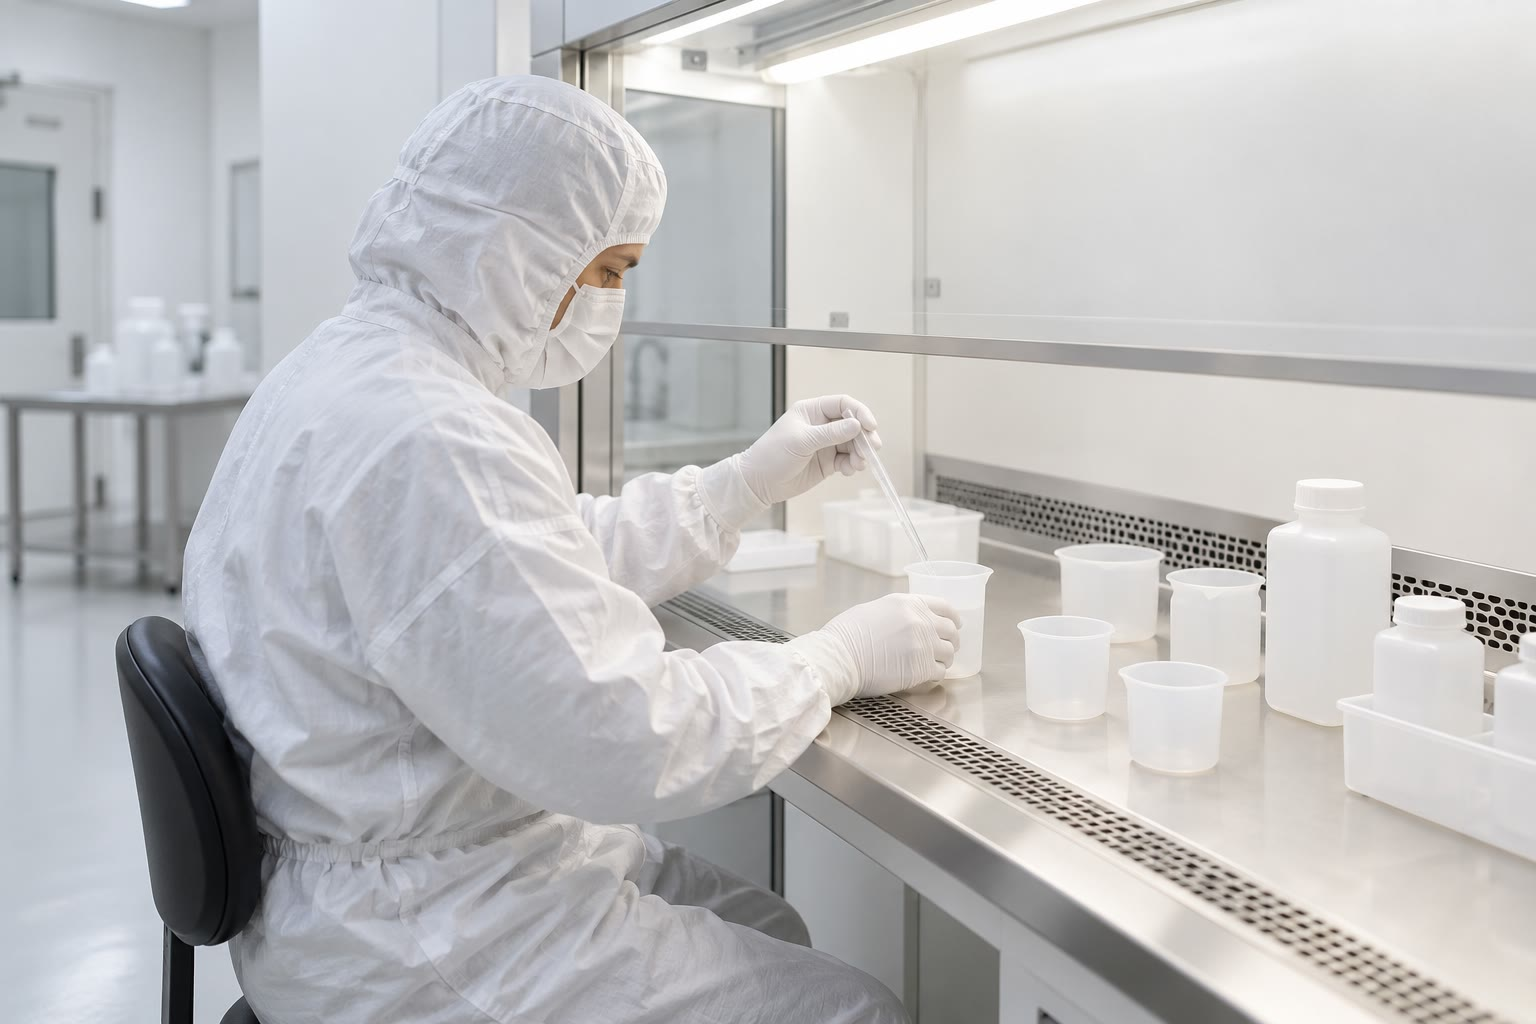
\includegraphics[width=\linewidth]{images/book4/ai/b2-clean-lab.jpg}

\smallskip
{\footnotesize 身着洁净服的工作人员在地球化学洁净实验室的层流
工作台前工作（AI 生成插图）。\par}
\end{minipage}
\end{inthelab}
% ledger: usgs:bhvo2-trace, usgs:bhvo2-origin

\section{练习}

\begin{exercise}[$\star$]\label{exo:b2:elements-in-the-earth:1}
夏威夷玄武岩 BHVO-2 含 0.5130\% \ce{K2O} 和 2.731\% \ce{TiO2}，
均为质量分数。取原子质量 K 39.10、Ti 47.87 和 O 16.00，求其
钾和钛的含量，单位为 ppm。
\end{exercise}

\begin{exercise}[$\star$]\label{exo:b2:elements-in-the-earth:2}
在\omterm{def:b2:elements-in-the-earth:bse}{全硅酸盐地球}中，$(X/\mathrm{Mg})$ 比值除以 CI 比值之后，
铝为 1.16，钠为 0.22，镍为 0.077，铱为
0.0029。这些元素的\omterm{def:b2:planet-formation-meteorites:condensation}{凝聚温度}分别为 1653、958、1353
和 \qty{1603}{K}。求每种元素的\omterm{def:b2:elements-in-the-earth:goldschmidt}{戈尔德施密特分类}，
并解释各元素的亏损。
\end{exercise}

\begin{exercise}[$\star$]\label{exo:b2:elements-in-the-earth:3}
上陆壳含镧 \qty{31}{ppm}、镱 \qty{2.0}{ppm}；
\omterm{def:b2:elements-in-the-earth:ci}{CI 球粒陨石}中分别为 0.232 和 \qty{0.163}{ppm}。计算\omterm{def:b2:planet-formation-meteorites:chondrule}{球粒陨石}标准化值
及 $(\mathrm{La}/\mathrm{Yb})_N$。该比值
说明了地壳的什么特征？
\end{exercise}

\begin{exercise}[$\star$]\label{exo:b2:elements-in-the-earth:4}
上陆壳含钐 4.7、铕 1.0、钆 \qty{4.0}{ppm}，
\omterm{def:b2:elements-in-the-earth:ci}{CI 球粒陨石}中分别为 0.145、0.0546 和 \qty{0.198}{ppm}。
计算 $\mathrm{Eu}/\mathrm{Eu}^*$。哪种矿物可以解释这一结果？
\end{exercise}

\begin{exercise}[$\star\star$]\label{exo:b2:elements-in-the-earth:5}
一种石榴子石辉石岩由 65\% 的单斜辉石、18\% 的石榴子石以及
17\% 的橄榄石、斜方辉石和尖晶石组成。镧的分配系数分别为
0.058、0.001 和 0.001，镥的分配系数分别为 0.53、5.8 和 0.18。
计算总分配系数。该岩石中哪种元素为\omterm{def:b2:elements-in-the-earth:partition}{相容元素}？
哪种矿物占据该岩石中大部分的镥？
\end{exercise}

\begin{exercise}[$\star\star$]\label{exo:b2:elements-in-the-earth:6}
\omterm{def:b2:elements-in-the-earth:bse}{全硅酸盐地球}中镁含量为 22.8\%，钠为 \qty{2670}{ppm}，
镍为 \qty{1960}{ppm}；\omterm{def:b2:elements-in-the-earth:ci}{CI 球粒陨石}中分别为 9.587\%、
\qty{5010}{ppm} 和 \qty{10640}{ppm}。计算钠和镍以镁标准化的 CI 比值。
两种元素的\omterm{def:b2:planet-formation-meteorites:condensation}{凝聚温度}均在 \qty{1000}{K} 附近或更高；为何
镍的亏损更为明显？
\end{exercise}

\begin{exercise}[$\star\star$]\label{exo:b2:elements-in-the-earth:7}
单斜辉石从成分为平均 MORB 的熔体中结晶，
该熔体含镧 \qty{5.21}{ppm}、镥 \qty{0.53}{ppm}。其分配系数，
镧为 0.058，镥为 0.53。计算其镧和镥的含量，
以及晶体与熔体中 $(\mathrm{La}/\mathrm{Lu})_N$ 之比，
（CI 中：La 0.232，Lu \qty{0.0237}{ppm}）。
\end{exercise}

\begin{exercise}[$\star\star$]\label{exo:b2:elements-in-the-earth:8}
以\omterm{def:b2:elements-in-the-earth:bse}{原始地幔}标准化（Nb \qty{0.658}{ppm}，La \qty{0.648}{ppm}），
计算上陆壳（Nb 12，
La \qty{31}{ppm}）、夏威夷玄武岩（18.10，\qty{15.20}{ppm}）和平均 MORB（
5.24，\qty{5.21}{ppm}）的 $(\mathrm{Nb}/\mathrm{La})_N$。其中哪一个带有俯冲带的特征？
\end{exercise}

\begin{exercise}[$\star\star$]\label{exo:b2:elements-in-the-earth:9}
钾和铀都是高度\omterm{def:b2:elements-in-the-earth:partition}{不相容元素}。计算 K/U 的质量比，分别在
\omterm{def:b2:elements-in-the-earth:bse}{原始地幔}（K \qty{240}{ppm}，U \qty{0.0203}{ppm}）、平均 MORB
（\qty{0.160}{\percent} \ce{K2O}，U \qty{0.119}{ppm}）和上陆壳
（\qty{2.80}{\percent} \ce{K2O}，U \qty{2.7}{ppm}）中求得，所用
$\mathrm{K}/\ce{K2O} = 0.830$（质量比）。该比值几乎不变说明了什么？
为何 K/U 可用于估算行星的钾含量？
\end{exercise}

\begin{exercise}[$\star\star\star$]\label{exo:b2:elements-in-the-earth:10}
一小份熔体与练习
5 中的石榴子石辉石岩处于平衡。证明：对于两种元素，比值
$(C_1/C_2)_{\mathrm{melt}}/(C_1/C_2)_{\mathrm{rock}}$ 等于
$\bar D_2/\bar D_1$。计算镧和镥的该比值，并解释为何
含石榴子石的地幔所产生的熔体具有陡峭的稀土配分模式。
\end{exercise}

\begin{exercise}[$\star\star\star$]\label{exo:b2:elements-in-the-earth:11}
一平均 MORB（Th \qty{0.404}{ppm}，Nb \qty{5.24}{ppm}）
混染了上陆壳（Th \qty{10.5}{ppm}，Nb \qty{12}{ppm}）：以质量分数 $f$ 计的地壳
与 $1-f$ 的玄武岩相混合。证明：混合物的浓度关于 $f$ 为线性，
但其 Th/Nb 比值并非线性。求使 Th/Nb 达到 0.2 的 $f$，
并求 $f = 0.1$ 时的比值。
\end{exercise}

\begin{exercise}[$\star\star\star$]\label{exo:b2:elements-in-the-earth:12}
去除水、碳或不含铝、镁的金属地核，
不会改变其余部分的 Al/Mg 比值，试证明之。在\omterm{def:b2:elements-in-the-earth:bse}{全硅酸盐地球}中，
$(\mathrm{Al}/\mathrm{Mg})$ 为 CI 值的 1.16 倍。
若地球保留了全部铝，则\omterm{def:b2:elements-in-the-earth:bse}{全硅酸盐地球}中缺失的\omterm{def:b2:planet-formation-meteorites:chondrule}{球粒陨石}镁占
的比例为多少？若以镁归一化的硅比值为 0.83，
则按同一假设，\omterm{def:b2:planet-formation-meteorites:chondrule}{球粒陨石}硅中缺失的比例为
多少？
\end{exercise}

\section{问题：用球粒陨石称量地核}

\begin{problem}[{周末问题——由 CI 球粒陨石重建整体地球、
地幔与地核，并称量地核}]
\label{pb:b2:elements-in-the-earth:1}
一位行星地球化学家希望不借助地震学，仅从化学角度称量地核。
她取 \omterm{def:b2:elements-in-the-earth:ci}{CI 球粒陨石}作为起始物质（Mg
\qty{95870}{ppm}、Al 8500、Si \num{106500}、Fe \num{182800}、Ni
\qty{10640}{ppm}），以\omterm{def:b2:elements-in-the-earth:bse}{原始地幔}代表硅酸盐地球（MgO 37.8、FeO
8.05、NiO 0.25\%；Mg 22.8、Si 21.0\%），并给出一个模型地核，其成分为 85.5
\% Fe、5.2\% Ni 和 6.0\% Si。原子质量：Mg 24.31、
Si 28.09、Fe 55.85、Ni 58.69、O 16.00。地球质量
\qty{5.972e24}{kg}.

\medskip\noindent\textbf{第一部分——\omterm{def:b2:planet-formation-meteorites:chondrule}{球粒陨石}起点。}
\begin{enumerate}
\item 计算 \omterm{def:b2:elements-in-the-earth:ci}{CI 球粒陨石}的质量比 Fe/Mg、Ni/Mg、Si/Mg 和 Al/Mg。
\item 将 Fe/Si 换算为原子比。太阳光球层的光谱学测量
给出每个硅原子对应 0.81 个铁原子：该比较是否合理？
\item \omterm{def:b2:elements-in-the-earth:ci}{CI 球粒陨石}含 2.1\% 的氢和 3.5\% 的碳，它们以结合态存在于含水矿物
与有机化合物中，这些物质未被地球保留。为何
第 1 题中的比值无需因这一损失加以修正？
\item 为何镁适宜作为地核问题的参考元素，而
铁却不能充当？
\item 镍、镁、铁和硅的\omterm{def:b2:planet-formation-meteorites:condensation}{凝聚温度}彼此相差在 \qty{50}{K} 之内
（分别为 1353、1336、1334 和 \qty{1310}{K}）。这一事实为何支持
整体地球保留了其\omterm{def:b2:planet-formation-meteorites:chondrule}{球粒陨石}比值的假设？第 1 题中哪一比值
偏离了这一组，本章对此有何说明？
\end{enumerate}

\noindent\textbf{第二部分——硅酸盐地球。}
\begin{enumerate}[resume]
\item 将\omterm{def:b2:elements-in-the-earth:bse}{原始地幔}中的 FeO 和 NiO 换算为 Fe 和 Ni。
\item 计算硅酸盐地球中的 Fe/Mg 和 Ni/Mg。
\item 在镁含量不变的条件下，\omterm{def:b2:planet-formation-meteorites:chondrule}{球粒陨石}中的 Fe 和 Ni
有多大比例在硅酸盐地球中缺失？
\item 对铱（\omterm{def:b2:elements-in-the-earth:bse}{原始地幔} \qty{3.2}{ppb}，CI
\qty{0.470}{ppm}）作同样计算，得到的缺失比例为 99.7\%。为何其比例高于
镍，而镍的比例又高于铁？
\item 铁在硅酸盐地球中处于何处？为何铁没有全部进入
地核？
\end{enumerate}

\noindent\textbf{第三部分——称量地核。}
\begin{enumerate}[resume]
\item 以地核质量分数 $x$ 写出地球的铁质量平衡式，并
推导\cref{prop:b2:elements-in-the-earth:core}。
\item 计算 $y = x/(1-x)$，并由铁求出 $x$。
\item 由镍作同样计算。
\item 两个估计值并不完全一致。用最小二乘法将二者合并：
使 $\sum (a_iy - b_i)^2$ 最小，其中 $a_i y = b_i$ 为
第 12 题与第 13 题中的两个方程，并给出最优的 $y$ 与 $x$。
\item 为何最小二乘值与铁的估计值如此接近？
\item 由这两个方程，计算使二者严格成立的地核 Fe/Ni 比值，
并与模型地核作比较。
\item 给出地核的质量。
\end{enumerate}

\noindent\textbf{第四部分——检验与推论。}
\begin{enumerate}[resume]
\item 地震学给出地核占地球质量的 32.5\%。化学估计值与之相差
多少个百分点？
\item 若地核占 32.5\%，则地核需含多少铁，
方能闭合铁平衡？这与地核中轻元素占
10\% 是否相容？
\item 模型地核中除 Fe 和 Ni 之外的元素占 9.3\%。哪些
轻元素可能是候选者，本章中有何证据支持硅？
\item 利用第 14 题的 $y$，计算使整体地球的 Si/Mg 恰为\omterm{def:b2:planet-formation-meteorites:chondrule}{球粒陨石}比值时
地核所需的硅含量。
\item 与模型中的 6\% 作比较。结合前一章，
试说明为何地球中可能完全缺失部分硅。
\item 模型地核含金 \qty{0.5}{ppm}，\omterm{def:b2:elements-in-the-earth:bse}{原始地幔}含金
\qty{1}{ppb}。若地核占 32.5\%，则地球的金有多大比例
位于地核中？
\item 给出仅由化学方法得到的地球地核质量分数，
这是本题的关键结果。
\end{enumerate}
\end{problem}
% ledger: lodders:ci-table, lodders:ci-h-photo, ms95:pm-oxides, ms95:pm-trace, mcd03:core, earth:mass, badro:core, lodders:tc-table
